\synctex=1
\documentclass[11pt,aspectratio=169]{beamer}

\usepackage[T1]{fontenc}
\usepackage[french,provide=*]{babel}
\usepackage{amsmath,amssymb,amsfonts}
\usepackage{mathtools}
\usepackage{bm}
\usepackage{tikz}
\usetikzlibrary{arrows.meta,positioning,calc}

% Couleurs pour les graphiques
\definecolor{darkblue}{RGB}{0,51,102}
\definecolor{lightblue}{RGB}{230,240,250}
\definecolor{darkgreen}{RGB}{0,102,51}
\definecolor{darkred}{RGB}{139,0,0}

% Police serif pour les mathématiques
\usefonttheme[onlymath]{serif}

% Git hash
\usepackage{xstring}
\usepackage{catchfile}
\immediate\write18{git rev-parse HEAD > git.hash}
\CatchFileDef{\HEAD}{git.hash}{\endlinechar=-1}
\newcommand{\gitrevision}{\StrLeft{\HEAD}{7}}

\usepackage{ccicons}

% Pied de page personnalisé
\setbeamertemplate{footline}{
  \hfill\vspace*{1pt}\href{https://creativecommons.org/publicdomain/zero/1.0/deed.fr}{\cczero}\enspace\href{https://github.com/stepan-a/time-series}{\gitrevision}\enspace--\enspace\insertframenumber/\inserttotalframenumber\enspace--\enspace\today\enspace}

% Supprimer la barre de navigation
\setbeamertemplate{navigation symbols}{}

% Commandes personnalisées
\newcommand{\E}{\mathbb{E}}
\newcommand{\Var}{\mathbb{V}}
\newcommand{\Cov}{\mathrm{Cov}}
\newcommand{\Corr}{\mathrm{Corr}}
\newcommand{\R}{\mathbb{R}}
\newcommand{\Z}{\mathbb{Z}}
\newcommand{\N}{\mathbb{N}}

\title{Modèles état-mesure et filtre de Kalman}
\author{}
\date{}
\institute{}

\AtBeginSection[]
{
  \begin{frame}
    \frametitle{Plan}
    \tableofcontents[currentsection]
  \end{frame}
}

\begin{document}

\begin{frame}
\titlepage
\end{frame}

\begin{frame}{Plan}
\tableofcontents
\end{frame}

%==============================================================================
\section{Introduction aux modèles état-mesure}
%==============================================================================

\begin{frame}{Motivation}

\begin{itemize}

\item Les modèles état-mesure constituent un cadre général permettant de :
  \begin{itemize}
  \item unifier de nombreux modèles de séries temporelles (ARMA, tendances, saisonnalité),
  \item traiter les observations manquantes de manière naturelle,
  \item estimer des composantes non observables (tendance, cycle),
  \item effectuer des prévisions optimales via le filtre de Kalman.\newline
  \end{itemize}

\item \textbf{Idée centrale :} Distinguer ce que l'on \textbf{observe} (équation de mesure) de la \textbf{dynamique latente} (équation d'état) qui gouverne le système.

\end{itemize}

\end{frame}

\begin{frame}{Formulation générale}

\begin{itemize}

\item \textbf{Équation de mesure} (observation) :
  \[
  \bm{y}_t = \bm{Z}_t \bm{\alpha}_t + \bm{d}_t + \bm{\varepsilon}_t, \quad \bm{\varepsilon}_t \sim N(\bm{0}, \bm{H}_t)
  \]\newline

\item \textbf{Équation d'état} (transition) :
  \[
  \bm{\alpha}_t = \bm{T}_t \bm{\alpha}_{t-1} + \bm{c}_t + \bm{R}_t \bm{\eta}_t, \quad \bm{\eta}_t \sim N(\bm{0}, \bm{Q}_t)
  \]\newline

\item \textbf{Dimensions :} $\bm{y}_t \in \R^p$ (observations), $\bm{\alpha}_t \in \R^m$ (état), $\bm{\varepsilon}_t \in \R^p$, $\bm{\eta}_t \in \R^r$.

\end{itemize}

\end{frame}

\begin{frame}{Notations et hypothèses}

\begin{itemize}

\item \textbf{Matrices du système :}
  \begin{itemize}
  \item $\bm{Z}_t$ : matrice de mesure $(p \times m)$,
  \item $\bm{T}_t$ : matrice de transition $(m \times m)$,
  \item $\bm{R}_t$ : matrice de sélection des perturbations $(m \times r)$,
  \item $\bm{H}_t$ : matrice de variance des erreurs de mesure $(p \times p)$,
  \item $\bm{Q}_t$ : matrice de variance des perturbations d'état $(r \times r)$,
  \item $\bm{d}_t$, $\bm{c}_t$ : termes déterministes.\newline
  \end{itemize}

\item \textbf{Hypothèses fondamentales :}
  \begin{itemize}
  \item $\E[\bm{\varepsilon}_t] = \bm{0}$, $\E[\bm{\eta}_t] = \bm{0}$,
  \item $\bm{\varepsilon}_t$ et $\bm{\eta}_s$ sont indépendants pour tout $t, s$,
  \item condition initiale : $\bm{\alpha}_0 \sim N(\bm{a}_0, \bm{P}_0)$,
  \item $\bm{\alpha}_0$ est indépendant de $\bm{\varepsilon}_t$ et $\bm{\eta}_t$ pour tout $t \geq 1$.
  \end{itemize}

\end{itemize}

\end{frame}

\begin{frame}{Représentation graphique}

\begin{center}
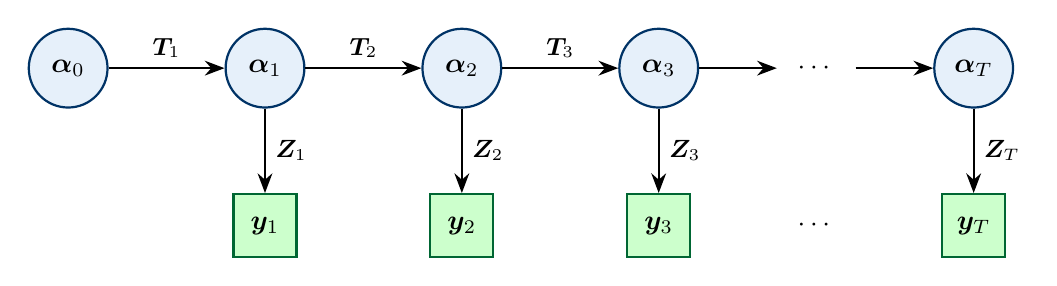
\begin{tikzpicture}[
    state/.style={circle, draw=darkblue, fill=lightblue, thick, minimum size=1cm},
    obs/.style={rectangle, draw=darkgreen, fill=green!20, thick, minimum size=0.8cm},
    arrow/.style={-{Stealth[length=2.5mm]}, thick}
]
    \node[state] (a0) at (-2.5,0) {$\bm{\alpha}_0$};
    \node[state] (a1) at (0,0) {$\bm{\alpha}_1$};
    \node[state] (a2) at (2.5,0) {$\bm{\alpha}_2$};
    \node[state] (a3) at (5,0) {$\bm{\alpha}_3$};
    \node at (7,0) {$\cdots$};
    \node[state] (aT) at (9,0) {$\bm{\alpha}_T$};

    \node[obs] (y1) at (0,-2) {$\bm{y}_1$};
    \node[obs] (y2) at (2.5,-2) {$\bm{y}_2$};
    \node[obs] (y3) at (5,-2) {$\bm{y}_3$};
    \node at (7,-2) {$\cdots$};
    \node[obs] (yT) at (9,-2) {$\bm{y}_T$};

    \draw[arrow] (a0) -- node[above, font=\small] {$\bm{T}_1$} (a1);
    \draw[arrow] (a1) -- node[above, font=\small] {$\bm{T}_2$} (a2);
    \draw[arrow] (a2) -- node[above, font=\small] {$\bm{T}_3$} (a3);
    \draw[arrow] (a3) -- (6.5,0);
    \draw[arrow] (7.5,0) -- (aT);

    \draw[arrow] (a1) -- node[right, font=\small] {$\bm{Z}_1$} (y1);
    \draw[arrow] (a2) -- node[right, font=\small] {$\bm{Z}_2$} (y2);
    \draw[arrow] (a3) -- node[right, font=\small] {$\bm{Z}_3$} (y3);
    \draw[arrow] (aT) -- node[right, font=\small] {$\bm{Z}_T$} (yT);
\end{tikzpicture}
\end{center}

Les états forment une \textbf{chaîne de Markov}, les observations sont conditionnellement indépendantes sachant les états.

\end{frame}

%==============================================================================
\section{Exemples de représentations état-mesure}
%==============================================================================

\begin{frame}{Exemple 1 : modèle de niveau local}

\begin{itemize}

\item Marche aléatoire avec bruit de mesure :
  \[
  y_t = \mu_t + \varepsilon_t, \quad \varepsilon_t \sim N(0, \sigma_\varepsilon^2)
  \]
  \[
  \mu_t = \mu_{t-1} + \eta_t, \quad \eta_t \sim N(0, \sigma_\eta^2)
  \]\newline

\item \textbf{Représentation état-mesure :} État $\alpha_t = \mu_t$ (scalaire, $m = 1$).
  \[
  Z = 1, \quad T = 1, \quad R = 1, \quad H = \sigma_\varepsilon^2, \quad Q = \sigma_\eta^2, \quad d = c = 0
  \]\newline

\item Ce modèle décompose la série en une \textbf{tendance stochastique} $\mu_t$ et un \textbf{bruit de mesure} $\varepsilon_t$.

\end{itemize}

\end{frame}

\begin{frame}{Exemple 2 : tendance linéaire locale}

\begin{itemize}

\item Le modèle s'écrit :
  \[
  y_t = \mu_t + \varepsilon_t, \quad \mu_t = \mu_{t-1} + \nu_{t-1} + \eta_t, \quad \nu_t = \nu_{t-1} + \zeta_t
  \]\newline

\item \textbf{Représentation état-mesure :} Vecteur d'état $\bm{\alpha}_t = (\mu_t, \nu_t)'$.
  \[
  \bm{Z} = \begin{pmatrix} 1 & 0 \end{pmatrix}, \quad
  \bm{T} = \begin{pmatrix} 1 & 1 \\ 0 & 1 \end{pmatrix}, \quad
  \bm{R} = \begin{pmatrix} 1 & 0 \\ 0 & 1 \end{pmatrix}
  \]
  \[
  H = \sigma_\varepsilon^2, \quad
  \bm{Q} = \begin{pmatrix} \sigma_\eta^2 & 0 \\ 0 & \sigma_\zeta^2 \end{pmatrix}
  \]

\end{itemize}

\end{frame}

\begin{frame}{Exemple 3 : processus AR(1)}

\begin{itemize}

\item Le modèle AR(1) :
  \[
  y_t = \phi y_{t-1} + \eta_t, \quad \eta_t \sim N(0, \sigma^2), \quad |\phi| < 1
  \]\newline

\item \textbf{Représentation état-mesure :} État $\alpha_t = y_t$.
  \begin{itemize}
  \item Équation de mesure : $y_t = \alpha_t$ (observation parfaite, $H = 0$),
  \item Équation d'état : $\alpha_t = \phi \alpha_{t-1} + \eta_t$.
  \end{itemize}
  Matrices : $Z = 1$, $T = \phi$, $R = 1$, $H = 0$, $Q = \sigma^2$.\newline

\item \textbf{Remarque :} Ici, l'état est directement observable ($H = 0$). Le filtre de Kalman se réduit à l'équation de récurrence de l'AR(1).

\end{itemize}

\end{frame}

\begin{frame}{Exemple 4 : processus AR($p$)}

\begin{itemize}

\item Le modèle AR($p$) :
  \[
  y_t = \phi_1 y_{t-1} + \phi_2 y_{t-2} + \cdots + \phi_p y_{t-p} + \eta_t
  \]\newline

\item \textbf{Représentation état-mesure} (forme compagnon) : vecteur d'état $\bm{\alpha}_t = (y_t, y_{t-1}, \ldots, y_{t-p+1})'$.
  \[
  \bm{Z} = \begin{pmatrix} 1 & 0 & \cdots & 0 \end{pmatrix}, \quad
  \bm{T} = \begin{pmatrix}
      \phi_1 & \phi_2 & \cdots & \phi_{p-1} & \phi_p \\
      1 & 0 & \cdots & 0 & 0 \\
      0 & 1 & \cdots & 0 & 0 \\
      \vdots & & \ddots & & \vdots \\
      0 & 0 & \cdots & 1 & 0
  \end{pmatrix}
  \]\newline

\item $\bm{R} = (1, 0, \ldots, 0)'$, $H = 0$, $Q = \sigma^2$.

\end{itemize}

\end{frame}

\begin{frame}{Exemple 5 : processus MA($q$)}

\begin{itemize}

\item Le modèle MA($q$) :
  \[
  y_t = \eta_t + \theta_1 \eta_{t-1} + \theta_2 \eta_{t-2} + \cdots + \theta_q \eta_{t-q}
  \]\newline

\item \textbf{Représentation état-mesure :} Vecteur d'état $\bm{\alpha}_t = (\eta_t, \eta_{t-1}, \ldots, \eta_{t-q})'$.
  \[
  \bm{Z} = \begin{pmatrix} 1 & \theta_1 & \theta_2 & \cdots & \theta_q \end{pmatrix}
  \]
  \[
  \bm{T} = \begin{pmatrix}
      0 & 0 & \cdots & 0 & 0 \\
      1 & 0 & \cdots & 0 & 0 \\
      0 & 1 & \cdots & 0 & 0 \\
      \vdots & & \ddots & & \vdots \\
      0 & 0 & \cdots & 1 & 0
  \end{pmatrix}, \quad
  \bm{R} = \begin{pmatrix} 1 \\ 0 \\ \vdots \\ 0 \end{pmatrix}
  \]\newline

\item $H = 0$, $Q = \sigma^2$.

\end{itemize}

\end{frame}

\begin{frame}{Exemple 6 : processus ARMA(1,1)}

\begin{itemize}

\item Le modèle ARMA(1,1) :
  \[
  y_t = \phi y_{t-1} + \eta_t + \theta \eta_{t-1}, \quad |\phi| < 1
  \]\newline

\item \textbf{Représentation état-mesure} (Harvey, 1989) : dimension $r = \max(1, 1+1) = 2$, vecteur d'état $\bm{\alpha}_t \in \R^2$.
  \[
  \bm{Z} = \begin{pmatrix} 1 & 0 \end{pmatrix}, \quad
  \bm{T} = \begin{pmatrix} \phi & 1 \\ 0 & 0 \end{pmatrix}, \quad
  \bm{R} = \begin{pmatrix} 1 \\ \theta \end{pmatrix}
  \]\newline

\item $H = 0$, $Q = \sigma^2$.

\end{itemize}

\end{frame}

\begin{frame}{Vérification : ARMA(1,1)}

\begin{itemize}

\item Avec $\bm{\alpha}_t = (\alpha_{1,t}, \alpha_{2,t})'$, l'\textbf{équation d'état} donne :
  \begin{align*}
  \alpha_{1,t} &= \phi \alpha_{1,t-1} + \alpha_{2,t-1} + \eta_t \\
  \alpha_{2,t} &= \theta \eta_t
  \end{align*}\newline

\item L'\textbf{observation} est $y_t = \alpha_{1,t}$.\newline

\item En substituant $\alpha_{2,t-1} = \theta \eta_{t-1}$ :
  \[
  y_t = \phi y_{t-1} + \theta \eta_{t-1} + \eta_t
  \]
  On retrouve bien le modèle ARMA(1,1). L'état $\alpha_{1,t}$ capture la dynamique AR, $\alpha_{2,t} = \theta\eta_t$ capture l'effet MA retardé.

\end{itemize}

\end{frame}

\begin{frame}{Exemple 7 : processus ARMA($p$,$q$) général}

\begin{itemize}

\item Pour $y_t - \sum_{i=1}^p \phi_i y_{t-i} = \eta_t + \sum_{j=1}^q \theta_j \eta_{t-j}$, on pose $r = \max(p, q+1)$ et $\bm{\alpha}_t \in \R^r$.\newline

\item Les matrices sont :
  \[
  \bm{T} = \begin{pmatrix}
      \phi_1 & 1 & 0 & \cdots & 0 \\
      \phi_2 & 0 & 1 & \cdots & 0 \\
      \vdots & & & \ddots & \\
      \phi_{r-1} & 0 & 0 & \cdots & 1 \\
      \phi_r & 0 & 0 & \cdots & 0
  \end{pmatrix}, \quad
  \bm{R} = \begin{pmatrix} 1 \\ \theta_1 \\ \vdots \\ \theta_{r-1} \end{pmatrix}
  \]
  avec $\phi_j = 0$ pour $j > p$ et $\theta_j = 0$ pour $j > q$.\newline

\item $\bm{Z} = (1, 0, \ldots, 0)$, $H = 0$, $Q = \sigma^2$.

\end{itemize}

\end{frame}

\begin{frame}{Exemple 8 : composante saisonnière}

\begin{itemize}

\item \textbf{Saisonnalité stochastique} (période $s$) :
  \[
  \gamma_t + \gamma_{t-1} + \cdots + \gamma_{t-s+1} = \omega_t, \quad \omega_t \sim N(0, \sigma_\omega^2)
  \]\newline

\item \textbf{Représentation état-mesure :} Vecteur d'état $\bm{\alpha}_t = (\gamma_t, \gamma_{t-1}, \ldots, \gamma_{t-s+2})'$ (dimension $s-1$).
  \[
  \bm{Z} = \begin{pmatrix} 1 & 0 & \cdots & 0 \end{pmatrix}, \quad
  \bm{T} = \begin{pmatrix}
      -1 & -1 & \cdots & -1 & -1 \\
      1 & 0 & \cdots & 0 & 0 \\
      0 & 1 & \cdots & 0 & 0 \\
      \vdots & & \ddots & & \vdots \\
      0 & 0 & \cdots & 1 & 0
  \end{pmatrix}
  \]\newline

\item $\bm{R} = (1, 0, \ldots, 0)'$, $Q = \sigma_\omega^2$.

\end{itemize}

\end{frame}

%==============================================================================
\section{Le filtre de Kalman}
%==============================================================================

\begin{frame}{Objectif du filtrage}

\begin{itemize}

\item Étant donné les observations $Y_t = \{y_1, y_2, \ldots, y_t\}$, on cherche à :
  \begin{itemize}
  \item \textbf{estimer} l'état courant $\bm{\alpha}_t$,
  \item \textbf{quantifier l'incertitude} de cette estimation,
  \item \textbf{mettre à jour} récursivement.
  \end{itemize}

\item \textbf{Estimateurs optimaux :}
  \begin{itemize}
  \item \textbf{Prédiction :} $\bm{a}_{t|t-1} = \E[\bm{\alpha}_t | Y_{t-1}]$ avec variance $\bm{P}_{t|t-1}$,
  \item \textbf{Filtrage :} $\bm{a}_{t|t} = \E[\bm{\alpha}_t | Y_t]$ avec variance $\bm{P}_{t|t}$.
  \end{itemize}

\item Sous les hypothèses gaussiennes, ces estimateurs sont les \textbf{BLUE} et coïncident avec l'espérance conditionnelle.

\end{itemize}

\end{frame}

\begin{frame}{Filtre de Kalman : vue d'ensemble}

\begin{center}
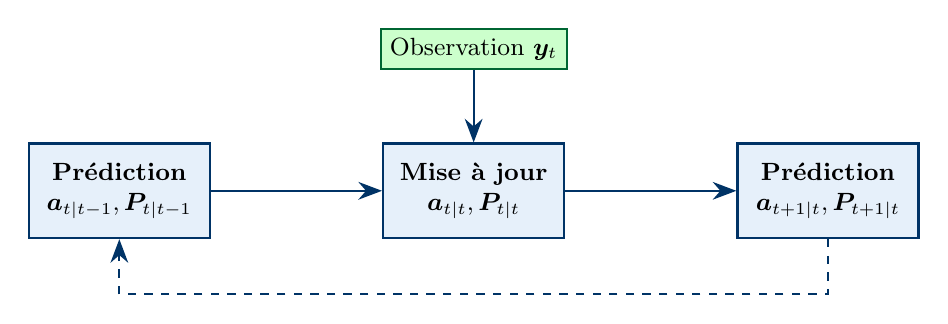
\begin{tikzpicture}[
    box/.style={rectangle, draw=darkblue, fill=lightblue, thick, minimum height=1.2cm, minimum width=2.3cm, align=center, font=\small},
    arrow/.style={-{Stealth[length=3mm]}, thick, darkblue}
]
    \node[box] (pred) at (0,0) {\textbf{Prédiction}\\$\bm{a}_{t|t-1}, \bm{P}_{t|t-1}$};
    \node[box] (update) at (4.5,0) {\textbf{Mise à jour}\\$\bm{a}_{t|t}, \bm{P}_{t|t}$};
    \node[box] (next) at (9,0) {\textbf{Prédiction}\\$\bm{a}_{t+1|t}, \bm{P}_{t+1|t}$};

    \node[rectangle, draw=darkgreen, fill=green!20, thick, font=\small] (obs) at (4.5,1.8) {Observation $\bm{y}_t$};

    \draw[arrow] (pred) -- (update);
    \draw[arrow] (update) -- (next);
    \draw[arrow] (obs) -- (update);

    \draw[arrow, dashed] (next.south) -- ++(0,-0.7) -| (pred.south);
\end{tikzpicture}
\end{center}

Le filtre alterne entre \textbf{prédiction} (projeter l'état via le modèle) et \textbf{correction} (incorporer la nouvelle observation).

\end{frame}

\begin{frame}{Équations du filtre de Kalman (1/2)}

\begin{itemize}

\item \textbf{Initialisation :} $\bm{a}_{0|0} = \bm{a}_0$, $\bm{P}_{0|0} = \bm{P}_0$.\newline

\item \textbf{Étape de prédiction :}
  \begin{align*}
  \bm{a}_{t|t-1} &= \bm{T}_t \bm{a}_{t-1|t-1} + \bm{c}_t \\
  \bm{P}_{t|t-1} &= \bm{T}_t \bm{P}_{t-1|t-1} \bm{T}_t' + \bm{R}_t \bm{Q}_t \bm{R}_t'
  \end{align*}

\end{itemize}

\end{frame}

\begin{frame}{Équations du filtre de Kalman (2/2)}

\begin{itemize}

\item \textbf{Étape de mise à jour :}
  \begin{align*}
  \bm{v}_t &= \bm{y}_t - \bm{Z}_t \bm{a}_{t|t-1} - \bm{d}_t & &\text{(innovation)} \\
  \bm{F}_t &= \bm{Z}_t \bm{P}_{t|t-1} \bm{Z}_t' + \bm{H}_t & &\text{(variance de l'innovation)} \\
  \bm{K}_t &= \bm{P}_{t|t-1} \bm{Z}_t' \bm{F}_t^{-1} & &\text{(gain de Kalman)} \\
  \bm{a}_{t|t} &= \bm{a}_{t|t-1} + \bm{K}_t \bm{v}_t \\
  \bm{P}_{t|t} &= (\bm{I} - \bm{K}_t \bm{Z}_t) \bm{P}_{t|t-1}
  \end{align*}

\end{itemize}

\end{frame}

\begin{frame}{Preuve : lemme préliminaire}

\begin{itemize}

\item \textbf{Lemme} (distribution conditionnelle gaussienne). Soit
  \[
  \begin{pmatrix} \bm{x} \\ \bm{y} \end{pmatrix} \sim N\!\left( \begin{pmatrix} \bm{\mu}_x \\ \bm{\mu}_y \end{pmatrix}, \begin{pmatrix} \bm{\Sigma}_{xx} & \bm{\Sigma}_{xy} \\ \bm{\Sigma}_{yx} & \bm{\Sigma}_{yy} \end{pmatrix} \right)
  \]
  Alors :
  \[
  \bm{x} | \bm{y} \sim N\!\left( \bm{\mu}_x + \bm{\Sigma}_{xy} \bm{\Sigma}_{yy}^{-1} (\bm{y} - \bm{\mu}_y), \; \bm{\Sigma}_{xx} - \bm{\Sigma}_{xy} \bm{\Sigma}_{yy}^{-1} \bm{\Sigma}_{yx} \right)
  \]\newline

\item On applique ce lemme avec $\bm{x} = \bm{\alpha}_t$ (état) et $\bm{y} = \bm{y}_t$ (observation), conditionnellement à $Y_{t-1}$.

\end{itemize}

\end{frame}

\begin{frame}{Preuve du lemme (1/2)}

\begin{itemize}

\item \textbf{Idée :} Décomposer $\bm{x}$ en une partie qui dépend linéairement de $\bm{y}$ et un résidu indépendant de $\bm{y}$.\newline

\item Posons $\bm{e} = \bm{x} - \bm{\mu}_x - \bm{\Sigma}_{xy} \bm{\Sigma}_{yy}^{-1} (\bm{y} - \bm{\mu}_y)$.\newline

\item \textbf{Covariance avec $\bm{y}$ :}
  \begin{align*}
  \Cov(\bm{e}, \bm{y}) &= \Cov(\bm{x}, \bm{y}) - \bm{\Sigma}_{xy} \bm{\Sigma}_{yy}^{-1} \Cov(\bm{y}, \bm{y}) \\
  &= \bm{\Sigma}_{xy} - \bm{\Sigma}_{xy} \bm{\Sigma}_{yy}^{-1} \bm{\Sigma}_{yy} = \bm{0}
  \end{align*}\newline

\item Puisque $(\bm{e}, \bm{y})$ est gaussien (transformation linéaire de $(\bm{x}, \bm{y})$), covariance nulle implique \textbf{indépendance}.

\end{itemize}

\end{frame}

\begin{frame}{Preuve du lemme (2/2)}

\begin{itemize}

\item On a donc $\bm{x} = \bm{\mu}_x + \bm{\Sigma}_{xy} \bm{\Sigma}_{yy}^{-1} (\bm{y} - \bm{\mu}_y) + \bm{e}$, avec $\bm{e} \perp\!\!\!\perp \bm{y}$.\newline

\item \textbf{Espérance conditionnelle :}
  \[
  \E[\bm{x} | \bm{y}] = \bm{\mu}_x + \bm{\Sigma}_{xy} \bm{\Sigma}_{yy}^{-1} (\bm{y} - \bm{\mu}_y) + \underbrace{\E[\bm{e}]}_{= \bm{0}} = \bm{\mu}_x + \bm{\Sigma}_{xy} \bm{\Sigma}_{yy}^{-1} (\bm{y} - \bm{\mu}_y)
  \]\newline

\item \textbf{Variance conditionnelle.} Puisque $\bm{e} = (\bm{x} - \bm{\mu}_x) - \bm{\Sigma}_{xy}\bm{\Sigma}_{yy}^{-1}(\bm{y} - \bm{\mu}_y)$ et $\Cov(\bm{e}, \bm{y}) = \bm{0}$ :
  \begin{align*}
  \Var[\bm{x} | \bm{y}] = \Var[\bm{e}] &= \Cov\!\big(\bm{e},\, (\bm{x}{-}\bm{\mu}_x) - \bm{\Sigma}_{xy}\bm{\Sigma}_{yy}^{-1}(\bm{y}{-}\bm{\mu}_y)\big) \\
  &= \Cov(\bm{e}, \bm{x}) + \bm{0} \\
  &= \bm{\Sigma}_{xx} - \bm{\Sigma}_{xy} \bm{\Sigma}_{yy}^{-1} \bm{\Sigma}_{yx} \qquad \square
  \end{align*}

\end{itemize}

\end{frame}

\begin{frame}{Preuve : étape de prédiction}

\begin{itemize}

\item \textbf{Hypothèse de récurrence :} $\bm{\alpha}_{t-1} | Y_{t-1} \sim N(\bm{a}_{t-1|t-1}, \bm{P}_{t-1|t-1})$.\newline

\item Par l'équation d'état : $\bm{\alpha}_t = \bm{T}_t \bm{\alpha}_{t-1} + \bm{c}_t + \bm{R}_t \bm{\eta}_t$.\newline

\item \textbf{Espérance conditionnelle :}
  \[
  \bm{a}_{t|t-1} = \E[\bm{\alpha}_t | Y_{t-1}] = \bm{T}_t \bm{a}_{t-1|t-1} + \bm{c}_t
  \]\newline

\item \textbf{Variance conditionnelle} (indépendance de $\bm{\eta}_t$ et $Y_{t-1}$) :
  \[
  \bm{P}_{t|t-1} = \Var[\bm{\alpha}_t | Y_{t-1}] = \bm{T}_t \bm{P}_{t-1|t-1} \bm{T}_t' + \bm{R}_t \bm{Q}_t \bm{R}_t'
  \]

\end{itemize}

\end{frame}

\begin{frame}{Preuve : distribution jointe}

\begin{itemize}

\item Par l'équation de mesure $\bm{y}_t = \bm{Z}_t \bm{\alpha}_t + \bm{d}_t + \bm{\varepsilon}_t$, la \textbf{distribution jointe} de $(\bm{\alpha}_t, \bm{y}_t)$ sachant $Y_{t-1}$ est :
  \[
  \begin{pmatrix} \bm{\alpha}_t \\ \bm{y}_t \end{pmatrix} \bigg| Y_{t-1} \sim N\!\left( \begin{pmatrix} \bm{a}_{t|t-1} \\ \bm{Z}_t \bm{a}_{t|t-1} + \bm{d}_t \end{pmatrix}, \begin{pmatrix} \bm{P}_{t|t-1} & \bm{P}_{t|t-1} \bm{Z}_t' \\ \bm{Z}_t \bm{P}_{t|t-1} & \bm{F}_t \end{pmatrix} \right)
  \]
  où $\bm{F}_t = \bm{Z}_t \bm{P}_{t|t-1} \bm{Z}_t' + \bm{H}_t$.\newline

\item \textbf{Calcul de la covariance :}
  \begin{align*}
  \Cov(\bm{\alpha}_t, \bm{y}_t | Y_{t-1}) &= \Cov(\bm{\alpha}_t, \bm{Z}_t \bm{\alpha}_t + \bm{\varepsilon}_t | Y_{t-1}) \\
  &= \bm{P}_{t|t-1} \bm{Z}_t' + \underbrace{\Cov(\bm{\alpha}_t, \bm{\varepsilon}_t)}_{= 0} = \bm{P}_{t|t-1} \bm{Z}_t'
  \end{align*}

\end{itemize}

\end{frame}

\begin{frame}{Preuve : étape de mise à jour}

\begin{itemize}

\item En appliquant le lemme avec $\bm{x} = \bm{\alpha}_t$ et $\bm{y} = \bm{y}_t$ :\newline

\item \textbf{Espérance conditionnelle :}
  \begin{align*}
  \bm{a}_{t|t} &= \E[\bm{\alpha}_t | Y_t] = \bm{a}_{t|t-1} + \bm{P}_{t|t-1} \bm{Z}_t' \bm{F}_t^{-1} (\bm{y}_t - \bm{Z}_t \bm{a}_{t|t-1} - \bm{d}_t) \\
  &= \bm{a}_{t|t-1} + \bm{K}_t \bm{v}_t
  \end{align*}
  où $\bm{K}_t = \bm{P}_{t|t-1} \bm{Z}_t' \bm{F}_t^{-1}$ est le \textbf{gain de Kalman}.\newline

\item \textbf{Variance conditionnelle :}
  \begin{align*}
  \bm{P}_{t|t} &= \bm{P}_{t|t-1} - \bm{P}_{t|t-1} \bm{Z}_t' \bm{F}_t^{-1} \bm{Z}_t \bm{P}_{t|t-1} \\
  &= (\bm{I} - \bm{K}_t \bm{Z}_t) \bm{P}_{t|t-1}
  \end{align*}

\end{itemize}

\end{frame}

\begin{frame}{Interprétation du gain de Kalman}

\begin{itemize}

\item Le gain $\bm{K}_t = \bm{P}_{t|t-1} \bm{Z}_t' \bm{F}_t^{-1}$ détermine le poids accordé à l'innovation :
  \[
  \bm{a}_{t|t} = \bm{a}_{t|t-1} + \bm{K}_t \bm{v}_t
  \]\newline

\item \textbf{Cas limites} (scalaire) :
  \begin{itemize}
  \item $H_t \to 0$ (mesure précise) : $K_t \to 1$ $\Rightarrow$ confiance totale à l'observation,
  \item $H_t \to \infty$ (mesure bruitée) : $K_t \to 0$ $\Rightarrow$ on garde la prédiction,
  \item $P_{t|t-1} \to 0$ (état bien connu) : $K_t \to 0$ $\Rightarrow$ pas d'information nouvelle.
  \end{itemize}

\end{itemize}

\end{frame}

\begin{frame}{Formule de Joseph}

\begin{itemize}

\item \textbf{Forme numériquement stable} pour $\bm{P}_{t|t}$ :
  \[
  \bm{P}_{t|t} = (\bm{I} - \bm{K}_t \bm{Z}_t) \bm{P}_{t|t-1} (\bm{I} - \bm{K}_t \bm{Z}_t)' + \bm{K}_t \bm{H}_t \bm{K}_t'
  \]
  Cette forme garantit que $\bm{P}_{t|t}$ reste symétrique et semi-définie positive.\newline

\item \textbf{Démonstration de l'équivalence.} En développant et utilisant $\bm{K}_t \bm{F}_t = \bm{P}_{t|t-1} \bm{Z}_t'$ :
  \begin{align*}
  &(\bm{I} - \bm{K}_t \bm{Z}_t) \bm{P}_{t|t-1} (\bm{I} - \bm{K}_t \bm{Z}_t)' + \bm{K}_t \bm{H}_t \bm{K}_t' \\
  &= \bm{P}_{t|t-1} - \bm{K}_t \bm{Z}_t \bm{P}_{t|t-1} - \bm{P}_{t|t-1} \bm{Z}_t' \bm{K}_t' + \bm{K}_t \bm{F}_t \bm{K}_t' \\
  &= \bm{P}_{t|t-1} - \bm{K}_t \bm{Z}_t \bm{P}_{t|t-1}
  \end{align*}

\end{itemize}

\end{frame}

\begin{frame}{Propriétés de l'innovation}

\begin{itemize}

\item L'\textbf{innovation} $\bm{v}_t = \bm{y}_t - \bm{Z}_t \bm{a}_{t|t-1} - \bm{d}_t$ est la partie de $\bm{y}_t$ non prévisible à partir de $Y_{t-1}$.\newline

\item \textbf{Propriétés fondamentales :}
  \begin{itemize}
  \item $\E[\bm{v}_t | Y_{t-1}] = 0$,
  \item $\Var[\bm{v}_t | Y_{t-1}] = \bm{F}_t$,
  \item $\Cov(\bm{v}_t, \bm{v}_s) = 0$ pour $t \neq s$.
  \end{itemize}

\item La suite $\{\bm{v}_t\}_{t=1}^T$ forme un \textbf{bruit blanc} (sous hypothèses gaussiennes). C'est essentiel pour le calcul de la vraisemblance et les diagnostics du modèle.

\end{itemize}

\end{frame}

\begin{frame}{Preuve : innovations non corrélées}

\begin{itemize}

\item Pour $s < t$, puisque $\bm{v}_s$ est $Y_s$-mesurable et $Y_s \subset Y_{t-1}$ :
  \[
  \Cov(\bm{v}_t, \bm{v}_s) = \E[\bm{v}_t \bm{v}_s'] \quad \text{(car $\E[\bm{v}_t] = \E[\bm{v}_s] = 0$)}
  \]\newline

\item Par la loi des espérances itérées :
  \begin{align*}
  \E[\bm{v}_t \bm{v}_s'] &= \E\!\left[\E[\bm{v}_t \bm{v}_s' | Y_{t-1}]\right] \\
  &= \E\!\left[\E[\bm{v}_t | Y_{t-1}] \bm{v}_s'\right] \quad \text{($\bm{v}_s$ est $Y_{t-1}$-mesurable)} \\
  &= \E[\bm{0} \cdot \bm{v}_s'] = \bm{0}
  \end{align*}

\end{itemize}

\end{frame}

\begin{frame}{Initialisation du filtre}

\begin{itemize}

\item \textbf{Cas stationnaire.} Si les valeurs propres de $\bm{T}$ ont un module $< 1$ :
  \[
  \bm{a}_{0|0} = \bm{0}, \quad \bm{P}_{0|0} \text{ solution de } \bm{P} = \bm{T} \bm{P} \bm{T}' + \bm{R} \bm{Q} \bm{R}'
  \]
  C'est une équation de Lyapunov, résolue par :
  \[
  \mathrm{vec}(\bm{P}) = (\bm{I} - \bm{T} \otimes \bm{T})^{-1} \mathrm{vec}(\bm{R} \bm{Q} \bm{R}')
  \]\newline

\item \textbf{Cas non stationnaire} (initialisation diffuse) :
  \[
  \bm{a}_{0|0} = \bm{0}, \quad \bm{P}_{0|0} = \kappa \bm{I} \quad \text{avec } \kappa \to \infty
  \]
  En pratique, on utilise le filtre de Kalman diffus exact (De Jong, 1991).

\end{itemize}

\end{frame}

%==============================================================================
\section{Le lisseur de Kalman}
%==============================================================================

\begin{frame}{Motivation du lissage}

\begin{itemize}

\item Le \textbf{filtrage} utilise $Y_t$ pour estimer $\bm{\alpha}_t$. Le \textbf{lissage} utilise \textbf{toute} l'information $Y_T = \{y_1, \ldots, y_T\}$ :
  \[
  \bm{a}_{t|T} = \E[\bm{\alpha}_t | Y_T], \quad \bm{P}_{t|T} = \Var[\bm{\alpha}_t | Y_T]
  \]

\end{itemize}

\begin{center}
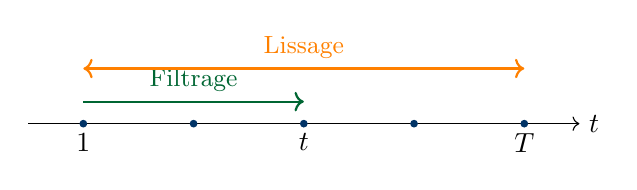
\begin{tikzpicture}[scale=0.7]
    \draw[->] (0,0) -- (10,0) node[right] {$t$};
    \foreach \x in {1,3,5,7,9} {\fill[darkblue] (\x,0) circle (2pt);}
    \node[below] at (1,0) {$1$};
    \node[below] at (5,0) {$t$};
    \node[below] at (9,0) {$T$};

    \draw[thick, darkgreen, ->] (1,0.4) -- (5,0.4);
    \node[above, darkgreen, font=\small] at (3,0.4) {Filtrage};

    \draw[thick, orange, <->] (1,1) -- (9,1);
    \node[above, orange, font=\small] at (5,1) {Lissage};
\end{tikzpicture}
\end{center}

Le lisseur exploite l'information future : $\bm{P}_{t|T} \leq \bm{P}_{t|t}$.

\end{frame}

\begin{frame}{Lisseur}

\begin{itemize}

\item \textbf{Initialisation :} $\bm{a}_{T|T}$, $\bm{P}_{T|T}$ (issus du filtre).\newline

\item \textbf{Récurrence arrière} pour $t = T-1, T-2, \ldots, 0$ :
  \begin{align*}
  \bm{J}_t &= \bm{P}_{t|t} \bm{T}_{t+1}' \bm{P}_{t+1|t}^{-1} & &\text{(gain de lissage)} \\
  \bm{a}_{t|T} &= \bm{a}_{t|t} + \bm{J}_t (\bm{a}_{t+1|T} - \bm{a}_{t+1|t}) \\
  \bm{P}_{t|T} &= \bm{P}_{t|t} + \bm{J}_t (\bm{P}_{t+1|T} - \bm{P}_{t+1|t}) \bm{J}_t'
  \end{align*}\newline

\item \textbf{Complexité :} une passe avant (filtre) + une passe arrière. Total : $O(Tm^3)$.

\end{itemize}

\end{frame}

\begin{frame}{Preuve du lisseur (1/2)}

\begin{itemize}

\item \textbf{Étape 1 :} Le couple $(\bm{\alpha}_t, \bm{\alpha}_{t+1})$ sachant $Y_t$ suit :
  \[
  \begin{pmatrix} \bm{\alpha}_t \\ \bm{\alpha}_{t+1} \end{pmatrix} \bigg| Y_t \sim N\!\left( \begin{pmatrix} \bm{a}_{t|t} \\ \bm{a}_{t+1|t} \end{pmatrix}, \begin{pmatrix} \bm{P}_{t|t} & \bm{P}_{t|t}\bm{T}_{t+1}' \\ \bm{T}_{t+1}\bm{P}_{t|t} & \bm{P}_{t+1|t} \end{pmatrix} \right)
  \]
  car $\Cov(\bm{\alpha}_t, \bm{\alpha}_{t+1}|Y_t) = \Cov(\bm{\alpha}_t, \bm{T}_{t+1}\bm{\alpha}_t|Y_t) = \bm{P}_{t|t}\bm{T}_{t+1}'$.\newline

\item \textbf{Étape 2 :} Par le lemme gaussien :
  \[
  \bm{\alpha}_t | (\bm{\alpha}_{t+1}, Y_t) \sim N\!\left( \bm{a}_{t|t} + \bm{J}_t (\bm{\alpha}_{t+1} - \bm{a}_{t+1|t}), \; \bm{P}_{t|t} - \bm{J}_t \bm{P}_{t+1|t} \bm{J}_t' \right)
  \]
  où $\bm{J}_t = \bm{P}_{t|t} \bm{T}_{t+1}' \bm{P}_{t+1|t}^{-1}$.

\end{itemize}

\end{frame}

\begin{frame}{Preuve du lisseur (2/2)}

\begin{itemize}

\item \textbf{Étape 3 :} Espérance lissée (loi des espérances itérées) :
  \begin{align*}
  \bm{a}_{t|T} &= \E[\bm{\alpha}_t | Y_T] = \E\!\left[\E[\bm{\alpha}_t | \bm{\alpha}_{t+1}, Y_t] | Y_T\right] \\
  &= \E\!\left[\bm{a}_{t|t} + \bm{J}_t (\bm{\alpha}_{t+1} - \bm{a}_{t+1|t}) | Y_T\right] \\
  &= \bm{a}_{t|t} + \bm{J}_t (\bm{a}_{t+1|T} - \bm{a}_{t+1|t})
  \end{align*}\newline

\item \textbf{Étape 4 :} Variance lissée (loi de la variance totale) :
  \begin{align*}
  \bm{P}_{t|T} &= \E\!\left[\Var[\bm{\alpha}_t | \bm{\alpha}_{t+1}, Y_t] | Y_T\right] + \Var\!\left[\E[\bm{\alpha}_t | \bm{\alpha}_{t+1}, Y_t] | Y_T\right] \\
  &= \bm{P}_{t|t} - \bm{J}_t \bm{P}_{t+1|t} \bm{J}_t' + \bm{J}_t \bm{P}_{t+1|T} \bm{J}_t' \\
  &= \bm{P}_{t|t} + \bm{J}_t(\bm{P}_{t+1|T} - \bm{P}_{t+1|t})\bm{J}_t'
  \end{align*}

\end{itemize}

\end{frame}

%==============================================================================
\section{Estimation par maximum de vraisemblance}
%==============================================================================

\begin{frame}{Paramètres à estimer}

\begin{itemize}

\item Les matrices du système dépendent de paramètres inconnus $\bm{\theta} = (\theta_1, \ldots, \theta_k)'$.\newline

\item \textbf{Exemple ARMA(1,1) :} $\bm{\theta} = (\phi, \theta, \sigma^2)'$.\newline

\item \textbf{Objectif :}
  \[
  \hat{\bm{\theta}}_{\mathrm{MV}} = \arg\max_{\bm{\theta}} \mathcal{L}(\bm{\theta}; Y_T)
  \]

\end{itemize}

\end{frame}

\begin{frame}{Décomposition de la vraisemblance}

\begin{itemize}

\item \textbf{Décomposition de l'erreur de prédiction :}
  \[
  f(y_1, \ldots, y_T; \bm{\theta}) = f(y_1; \bm{\theta}) \prod_{t=2}^{T} f(y_t | Y_{t-1}; \bm{\theta})
  \]\newline

\item Puisque $\bm{y}_t | Y_{t-1} \sim N(\bm{Z}_t \bm{a}_{t|t-1} + \bm{d}_t, \bm{F}_t)$, on a :
  \[
  f(\bm{y}_t | Y_{t-1}) = (2\pi)^{-p/2} |\bm{F}_t|^{-1/2} \exp\!\left( -\frac{1}{2} \bm{v}_t' \bm{F}_t^{-1} \bm{v}_t \right)
  \]

\end{itemize}

\end{frame}

\begin{frame}{Log-vraisemblance}

\begin{itemize}

\item La \textbf{log-vraisemblance} s'écrit :
  \[
  \boxed{\mathcal{L}(\bm{\theta}) = -\frac{pT}{2} \log(2\pi) - \frac{1}{2} \sum_{t=1}^{T} \log |\bm{F}_t| - \frac{1}{2} \sum_{t=1}^{T} \bm{v}_t' \bm{F}_t^{-1} \bm{v}_t}
  \]\newline

\item Pour évaluer $\mathcal{L}(\bm{\theta})$, il suffit d'exécuter le \textbf{filtre de Kalman} qui produit les innovations $\bm{v}_t$ et leurs variances $\bm{F}_t$.\newline

\item \textbf{Cas scalaire} ($p=1$) :
  \[
  \mathcal{L}(\bm{\theta}) = -\frac{T}{2} \log(2\pi) - \frac{1}{2} \sum_{t=1}^{T} \log F_t - \frac{1}{2} \sum_{t=1}^{T} \frac{v_t^2}{F_t}
  \]

\end{itemize}

\end{frame}

\begin{frame}{Vraisemblance concentrée}

\begin{itemize}

\item Si $\bm{Q} = \sigma^2 \bm{Q}^*$ et $\bm{H} = \sigma^2 \bm{H}^*$, la condition du premier ordre par rapport à $\sigma^2$ donne :
  \[
  \hat{\sigma}^2(\bm{\theta}^*) = \frac{1}{pT} \sum_{t=1}^{T} v_t^{*\prime} F_t^{*-1} v_t^*
  \]
  où les quantités $*$ sont calculées avec $\sigma^2 = 1$.\newline

\item On substitue $\hat{\sigma}^2$ dans la log-vraisemblance pour obtenir la \textbf{vraisemblance concentrée} $\mathcal{L}_c(\bm{\theta}^*)$ qui ne dépend plus de $\sigma^2$.\newline

\item Cela réduit la dimension du problème d'optimisation.

\end{itemize}

\end{frame}

\begin{frame}{Erreurs standard et diagnostics}

\begin{itemize}

\item \textbf{Matrice d'information de Fisher :}
  \[
  \mathcal{I}(\bm{\theta}) = -\frac{\partial^2 \mathcal{L}(\bm{\theta})}{\partial \bm{\theta}\, \partial \bm{\theta}'}
  \]
  Asymptotiquement : $\sqrt{T}(\hat{\bm{\theta}}_{\mathrm{MV}} - \bm{\theta}_0) \xrightarrow{d} N(\bm{0}, \mathcal{I}(\bm{\theta}_0)^{-1})$.\newline

\item \textbf{Diagnostics} sur les résidus standardisés $e_t = F_t^{-1/2} v_t$ :
  \begin{itemize}
  \item test de normalité : Jarque-Bera,
  \item test d'autocorrélation : Ljung-Box $Q(m) = T(T+2)\sum_{k=1}^m \frac{\hat{\rho}_k^2}{T-k}$,
  \item test ARCH sur $e_t^2$.
  \end{itemize}

\end{itemize}

\end{frame}

\begin{frame}{Sélection de modèles}

\begin{itemize}

\item \textbf{Critère d'Akaike} (AIC) :
  \[
  \mathrm{AIC} = -2\mathcal{L}(\hat{\bm{\theta}}) + 2k
  \]\newline

\item \textbf{Critère bayésien de Schwarz} (BIC) :
  \[
  \mathrm{BIC} = -2\mathcal{L}(\hat{\bm{\theta}}) + k \log(T)
  \]
  où $k$ est le nombre de paramètres et $T$ le nombre d'observations.\newline

\item On sélectionne le modèle qui \textbf{minimise} le critère. Le BIC pénalise davantage la complexité et est consistant.

\end{itemize}

\end{frame}

%==============================================================================
\section{Prévisions}
%==============================================================================

\begin{frame}{Types de prévisions}

\begin{itemize}

\item \textbf{Prévision à un pas :} $\hat{y}_{T+1|T} = \E[y_{T+1} | Y_T]$.\newline

\item \textbf{Prévision à $h$ pas :} $\hat{y}_{T+h|T} = \E[y_{T+h} | Y_T]$.\newline

\item \textbf{Stratégie :} Continuer les équations de prédiction au-delà de $T$, \textbf{sans} mise à jour.

\end{itemize}

\begin{center}
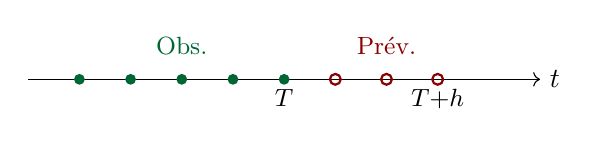
\begin{tikzpicture}[scale=0.65]
    \draw[->] (0,0) -- (10,0) node[right] {$t$};
    \foreach \x in {1,2,3,4,5} {\fill[darkgreen] (\x,0) circle (3pt);}
    \foreach \x in {6,7,8} {\draw[darkred, thick] (\x,0) circle (3pt);}
    \node[below, font=\small] at (5,0) {$T$};
    \node[below, font=\small] at (8,0) {$T{+}h$};
    \node[above, darkgreen, font=\small] at (3,0.3) {Obs.};
    \node[above, darkred, font=\small] at (7,0.3) {Prév.};
\end{tikzpicture}
\end{center}

\end{frame}

\begin{frame}{Équations de prévision}

\begin{itemize}

\item \textbf{Prévision de l'état} (pour $h \geq 1$) :
  \begin{align*}
  \bm{a}_{T+h|T} &= \bm{T}_{T+h} \bm{a}_{T+h-1|T} + \bm{c}_{T+h} \\
  \bm{P}_{T+h|T} &= \bm{T}_{T+h} \bm{P}_{T+h-1|T} \bm{T}_{T+h}' + \bm{R}_{T+h} \bm{Q}_{T+h} \bm{R}_{T+h}'
  \end{align*}
  Initialisation : $\bm{a}_{T|T}$, $\bm{P}_{T|T}$ (issus du filtre).\newline

\item \textbf{Prévision de l'observation :}
  \begin{align*}
  \hat{\bm{y}}_{T+h|T} &= \bm{Z}_{T+h} \bm{a}_{T+h|T} + \bm{d}_{T+h} \\
  \bm{F}_{T+h|T} &= \bm{Z}_{T+h} \bm{P}_{T+h|T} \bm{Z}_{T+h}' + \bm{H}_{T+h}
  \end{align*}

\end{itemize}

\end{frame}

\begin{frame}{Intervalles de prévision}

\begin{itemize}

\item \textbf{Intervalle à $(1-\alpha)\%$} (cas scalaire) :
  \[
  \hat{y}_{T+h|T} \pm z_{\alpha/2} \sqrt{F_{T+h|T}}
  \]
  Pour $\alpha = 0{,}05$ : $z_{0{,}025} \approx 1{,}96$.\newline

\item L'intervalle s'élargit avec $h$ car :
  \begin{itemize}
  \item l'incertitude sur l'état se propage,
  \item les chocs futurs s'accumulent.
  \end{itemize}

\item Pour un modèle stationnaire : $F_{T+h|T} \to$ variance inconditionnelle quand $h \to \infty$.

\end{itemize}

\end{frame}

\begin{frame}{Formules explicites (coefficients constants)}

\begin{itemize}

\item Si $\bm{T}_t = \bm{T}$, etc., l'\textbf{état prévu} est :
  \[
  \bm{a}_{T+h|T} = \bm{T}^h \bm{a}_{T|T} + \sum_{j=0}^{h-1} \bm{T}^j \bm{c}
  \]\newline

\item La \textbf{variance de prévision} est :
  \[
  \bm{P}_{T+h|T} = \bm{T}^h \bm{P}_{T|T} (\bm{T}')^h + \sum_{j=0}^{h-1} \bm{T}^j \bm{R} \bm{Q} \bm{R}' (\bm{T}')^j
  \]

\end{itemize}

\end{frame}

\begin{frame}{Exemple : prévision AR(1)}

\begin{itemize}

\item \textbf{Rappel :} $T = \phi$, $Z = 1$, $R = 1$, $H = 0$, $Q = \sigma^2$, état $\alpha_t = y_t$.\newline

\item Puisque $H = 0$ : $a_{T|T} = y_T$ et $P_{T|T} = 0$. Donc :
  \[
  \hat{y}_{T+h|T} = \phi^h y_T
  \]\newline

\item \textbf{Variance de prévision :} $P_{T+h|T} = \sigma^2 \sum_{j=0}^{h-1} \phi^{2j}$, soit :
  \[
  F_{T+h|T} = \sigma^2 \frac{1 - \phi^{2h}}{1 - \phi^2} \xrightarrow[h\to\infty]{} \frac{\sigma^2}{1 - \phi^2} = \Var[y_t]
  \]

\end{itemize}

\end{frame}

\begin{frame}{Exemple : prévision AR(1) -- illustration}

\begin{center}
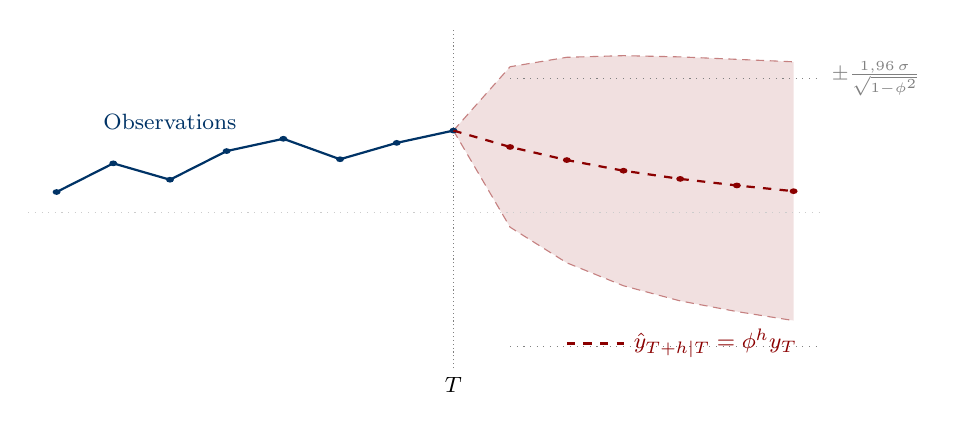
\begin{tikzpicture}[xscale=0.72, yscale=0.52]
  % Bande de confiance à 95%
  \fill[darkred!12]
    (8,2) -- (9,3.56) -- (10,3.79) -- (11,3.83) -- (12,3.80) -- (13,3.74) -- (14,3.68)
    -- (14,-2.64) -- (13,-2.42) -- (12,-2.16) -- (11,-1.79) -- (10,-1.23) -- (9,-0.36)
    -- (8,2) -- cycle;
  % Bornes IC
  \draw[darkred!50, densely dashed, thin]
    (8,2) -- (9,3.56) -- (10,3.79) -- (11,3.83) -- (12,3.80) -- (13,3.74) -- (14,3.68);
  \draw[darkred!50, densely dashed, thin]
    (8,2) -- (9,-0.36) -- (10,-1.23) -- (11,-1.79) -- (12,-2.16) -- (13,-2.42) -- (14,-2.64);
  % IC asymptotique (variance inconditionnelle)
  \draw[gray, dotted] (9,3.27) -- (14.5,3.27) node[right, font=\scriptsize] {$\pm\frac{1{,}96\,\sigma}{\sqrt{1-\phi^2}}$};
  \draw[gray, dotted] (9,-3.27) -- (14.5,-3.27);
  % Moyenne inconditionnelle
  \draw[gray!40, dotted] (0.5,0) -- (14.5,0);
  % Séparation T
  \draw[gray, densely dotted] (8,-3.8) -- (8,4.5);
  % Observations
  \draw[darkblue, thick]
    (1,0.5) -- (2,1.2) -- (3,0.8) -- (4,1.5) -- (5,1.8) -- (6,1.3) -- (7,1.7) -- (8,2.0);
  \foreach \x/\y in {1/0.5, 2/1.2, 3/0.8, 4/1.5, 5/1.8, 6/1.3, 7/1.7, 8/2.0}
    \fill[darkblue] (\x,\y) circle (2pt);
  % Prévision
  \draw[darkred, thick, dashed]
    (8,2.0) -- (9,1.6) -- (10,1.28) -- (11,1.02) -- (12,0.82) -- (13,0.66) -- (14,0.52);
  \foreach \x/\y in {9/1.6, 10/1.28, 11/1.02, 12/0.82, 13/0.66, 14/0.52}
    \fill[darkred] (\x,\y) circle (2pt);
  % Annotations
  \node[below, font=\footnotesize] at (8,-3.8) {$T$};
  \node[darkblue, font=\footnotesize, above] at (3,1.8) {Observations};
  \draw[darkred, thick, dashed] (10,-3.2) -- (11,-3.2)
    node[right, font=\footnotesize] {$\hat{y}_{T+h|T} = \phi^h y_T$};
\end{tikzpicture}
\end{center}

\vspace{-4pt}
{\small Paramètres : $\phi = 0{,}8$, $\sigma^2 = 1$, $y_T = 2$. La prévision décroît géométriquement et l'IC converge vers l'IC inconditionnel $\pm 1{,}96\,\sigma/\sqrt{1-\phi^2}$.}

\end{frame}

\begin{frame}{Exemple : prévision MA(1)}

\begin{itemize}

\item \textbf{Rappel :} $\bm{T} = \begin{pmatrix} 0 & 0 \\ 1 & 0 \end{pmatrix}$, $\bm{Z} = \begin{pmatrix} 1 & \theta \end{pmatrix}$, $\bm{R} = \begin{pmatrix} 1 \\ 0 \end{pmatrix}$, état $\bm{\alpha}_t = (\eta_t, \eta_{t-1})'$.\newline

\item La matrice $\bm{T}$ est \textbf{nilpotente} : $\bm{T}^2 = \bm{0}$. Pour $h \geq 1$ :
  \[
  \bm{Z}\bm{T}^h \bm{a}_{T|T} = \begin{cases} \theta\, a_{1,T|T} & \text{si } h = 1 \\ 0 & \text{si } h \geq 2 \end{cases}
  \]
  où $a_{1,T|T} = \E[\eta_T | Y_T]$ est l'innovation filtrée.\newline

\item \textbf{Variance de prévision} ($h \geq 2$) : $\bm{T}^h = \bm{0}$ et les seuls termes non nuls sont $j = 0, 1$ :
  \[
  F_{T+h|T} = \bm{Z}\!\left(\sigma^2 \bm{R}\bm{R}' + \sigma^2 \bm{T}\bm{R}\bm{R}'\bm{T}'\right)\!\bm{Z}' = \sigma^2(1 + \theta^2) = \Var[y_t]
  \]

\end{itemize}

\end{frame}

\begin{frame}{Exemple : prévision MA(1) -- illustration}

\begin{center}
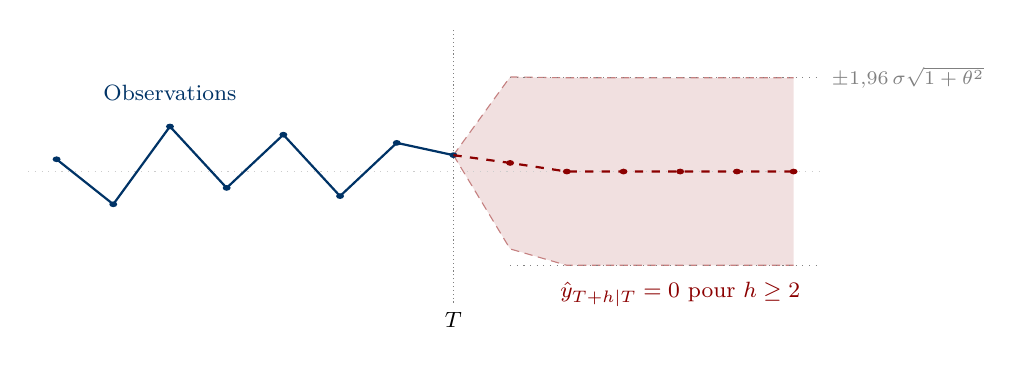
\begin{tikzpicture}[xscale=0.72, yscale=0.52]
  % Bande de confiance à 95%
  \fill[darkred!12]
    (8,0.4) -- (9,2.31) -- (10,2.29) -- (11,2.29) -- (12,2.29) -- (13,2.29) -- (14,2.29)
    -- (14,-2.29) -- (13,-2.29) -- (12,-2.29) -- (11,-2.29) -- (10,-2.29) -- (9,-1.89)
    -- (8,0.4) -- cycle;
  % Bornes IC
  \draw[darkred!50, densely dashed, thin]
    (8,0.4) -- (9,2.31) -- (10,2.29) -- (11,2.29) -- (12,2.29) -- (13,2.29) -- (14,2.29);
  \draw[darkred!50, densely dashed, thin]
    (8,0.4) -- (9,-1.89) -- (10,-2.29) -- (11,-2.29) -- (12,-2.29) -- (13,-2.29) -- (14,-2.29);
  % IC asymptotique (variance inconditionnelle)
  \draw[gray, dotted] (9,2.29) -- (14.5,2.29)
    node[right, font=\scriptsize] {$\pm 1{,}96\,\sigma\sqrt{1+\theta^2}$};
  \draw[gray, dotted] (9,-2.29) -- (14.5,-2.29);
  % Moyenne inconditionnelle
  \draw[gray!40, dotted] (0.5,0) -- (14.5,0);
  % Séparation T
  \draw[gray, densely dotted] (8,-3.2) -- (8,3.5);
  % Observations
  \draw[darkblue, thick]
    (1,0.3) -- (2,-0.8) -- (3,1.1) -- (4,-0.4) -- (5,0.9) -- (6,-0.6) -- (7,0.7) -- (8,0.4);
  \foreach \x/\y in {1/0.3, 2/-0.8, 3/1.1, 4/-0.4, 5/0.9, 6/-0.6, 7/0.7, 8/0.4}
    \fill[darkblue] (\x,\y) circle (2pt);
  % Prévision
  \draw[darkred, thick, dashed]
    (8,0.4) -- (9,0.21) -- (10,0) -- (11,0) -- (12,0) -- (13,0) -- (14,0);
  \foreach \x/\y in {9/0.21, 10/0, 11/0, 12/0, 13/0, 14/0}
    \fill[darkred] (\x,\y) circle (2pt);
  % Annotations
  \node[below, font=\footnotesize] at (8,-3.2) {$T$};
  \node[darkblue, font=\footnotesize, above] at (3,1.5) {Observations};
  \node[darkred, font=\footnotesize] at (12,-3)
    {$\hat{y}_{T+h|T} = 0$ pour $h \geq 2$};
\end{tikzpicture}
\end{center}

\vspace{-4pt}
{\small Paramètres : $\theta = 0{,}6$, $\sigma^2 = 1$. La prévision tombe à zéro dès $h = 2$ et l'IC atteint immédiatement la variance inconditionnelle $\sigma^2(1 + \theta^2)$.}

\end{frame}

\begin{frame}{Prévision ARMA($p$,$q$)}

\begin{itemize}

\item Pour un ARMA($p$,$q$), l'état filtré $\bm{a}_{T|T}$ contient toute l'information nécessaire à la prévision :
  \[
  \hat{y}_{T+h|T} = \bm{Z} \bm{T}^h \bm{a}_{T|T}
  \]\newline

\item \textbf{Exemple ARMA(1,1).} Avec $\bm{T} = \begin{pmatrix} \phi & 1 \\ 0 & 0 \end{pmatrix}$ :
  \[
  \bm{T}^h = \begin{pmatrix} \phi^h & \phi^{h-1} \\ 0 & 0 \end{pmatrix} \quad (h \geq 1)
  \]
  Donc : $\hat{y}_{T+h|T} = \phi^h a_{1,T|T} + \phi^{h-1} a_{2,T|T}$.

\end{itemize}

\end{frame}

\begin{frame}{Résumé}

\begin{itemize}

\item Les \textbf{modèles état-mesure} unifient ARMA, tendances et saisonnalité.\newline

\item Le \textbf{filtre de Kalman} fournit une estimation récursive optimale de l'état.\newline

\item Le \textbf{lisseur de Kalman} exploite toute l'information disponible.\newline

\item Le \textbf{maximum de vraisemblance} s'obtient via la décomposition de l'innovation.\newline

\item Les \textbf{prévisions} sont calculées par prolongation des équations de prédiction.\newline

\end{itemize}

\end{frame}

\end{document}
